\documentclass[11pt]{article}

\usepackage[margin=1in]{geometry}
\usepackage[T1]{fontenc}
\usepackage{lmodern}
\usepackage{microtype}
\usepackage{amsmath,amssymb}
\usepackage{booktabs}
\usepackage{enumitem}
\usepackage{caption}
\usepackage{float}
\usepackage{graphicx}
\usepackage{xcolor}
\usepackage[colorlinks=true,linkcolor=blue!50!black,citecolor=blue!50!black,urlcolor=blue!50!black]{hyperref}

\graphicspath{{../figures/}{figures/}}
\setlist{itemsep=0pt,topsep=2pt,parsep=0pt}
\usepackage[compact]{titlesec}
\titlespacing*{\section}{0pt}{8pt}{4pt}
\titlespacing*{\paragraph}{0pt}{4pt}{0.8em}
\setlength{\textfloatsep}{8pt plus 2pt}
\setlength{\floatsep}{6pt plus 2pt}
\setlength{\intextsep}{6pt plus 2pt}
\captionsetup{font=small,labelfont=bf}
\newcommand{\code}[1]{\texttt{\small #1}}

\title{\textbf{Do Time-Series Foundation Models Need Fine-Tuning?\\Wind Power Forecasting with PatchTST and Chronos}\\[2pt]
\large\emph{DATA612 PWS1 Group Project, Interim Report}}
\author{
\begin{tabular}{cc}
Simran Kharbanda & Tanmay Sharma \\
UID: 122283671 & UID: 121997234
\end{tabular}}
\date{October 29, 2026}

\begin{document}
\maketitle
\vspace{-2em}

\section{Introduction and problem statement}

Wind power is difficult to forecast because output follows wind speed, which varies from minute to minute.
Grid operators rely on short-term forecasts to schedule reserves and balance supply with demand, and forecast
errors are costly in both directions: over-forecasting leaves a shortfall that must be covered at spot prices,
and under-forecasting means reserve capacity is bought and not used.

A team building such a forecaster today has three options: train a small transformer on the farm's own history,
use a pretrained time-series foundation model as it is, or fine-tune that foundation model on the farm's data.
Which of these performs best, and at what cost in data and GPU time, is an open practical question, and it is
the one this project tests.

The task is as follows: for each of the 134 turbines in the SDWPF wind farm \cite{zhou2024sdwpf}, take the last
$L = 288$ ten-minute readings of active power (two days) and forecast the next $H$ readings, for $H = 6$, 36 and
64 (one hour, six hours, and about eleven hours). We compare PatchTST \cite{nie2023patchtst}, a transformer we
implement ourselves and train from scratch, against Chronos \cite{ansari2024chronos}, a pretrained T5 forecaster,
used three ways: zero-shot, fully fine-tuned, and fine-tuned with LoRA \cite{hu2022lora}. We stop at $H = 64$
because that is the longest horizon Chronos was trained for; going further would handicap it for reasons that
have nothing to do with our questions.

\section{Objectives and scope}

The three research questions from the proposal are unchanged.
\begin{description}
  \item[RQ1] Does PatchTST trained from scratch on SDWPF beat zero-shot Chronos?
  \item[RQ2] How much of the gap, in either direction, do full fine-tuning and LoRA close?
  \item[RQ3] How does each method behave with 5\%, 25\% and 100\% of the training data, and what does it cost in
  GPU hours and trainable parameters?
\end{description}

The work we have committed to is the full grid: \{PatchTST, Chronos full fine-tune, Chronos LoRA\} $\times$
\{5\%, 25\%, 100\% of the training data\} $\times$ 3 seeds, plus zero-shot Chronos and three baselines
(persistence, seasonal naive, LSTM), with every model scored by the same evaluation code on the same windows. We
also set ourselves a gate before any of this runs on wind data: our PatchTST had to reproduce the paper's ETTh1
numbers first. That gate has been passed (Section~\ref{sec:progress}).

Two things are optional enhancements: a multi-GPU fine-tune of the larger Chronos-T5-base, and a
spatial extension that gives PatchTST its neighbouring turbines as extra inputs. We are not using covariates such
as wind speed as model inputs (Chronos cannot take them, so the main comparison stays univariate), not going beyond
64 steps, and not using the extended two-year SDWPF release.

\section{Methodology}

\paragraph{Data and splits.} SDWPF \cite{zhou2024sdwpf} covers 134 turbines over 245 days at ten-minute
resolution: 4,727,520 rows, ten sensor columns, and the target \code{Patv} in kW. We follow the dataset paper's
cleaning rules. Negative power is clamped to zero. A reading is \emph{unknown} when power is at or below zero while
the wind is above 2.5\,m/s, or when any blade pitch angle exceeds $89^\circ$; it is \emph{abnormal} when the nacelle
direction is outside $\pm720^\circ$ or the wind direction outside $\pm180^\circ$; and it is \emph{missing} when
\code{Patv} is NaN. Flagged readings stay in the model inputs as real history, but they never count towards the
loss or the metrics.

The split is chronological and aligned to whole days: 171 days of training, 25 of validation, 49 of test. The 5\%
and 25\% subsets are the most recent 1,231 and 6,156 steps of the training period, nested, so a model trained on
25\% has seen everything the 5\% model saw. Forecast origins in validation and test sit every 36 steps, at 00:00,
06:00, 12:00 and 18:00, which gives 99 validation and 195 test origins per turbine, identical for every model.
Training windows use stride 1 and must lie entirely inside their subset. At evaluation time the history may reach
back into the previous period, but a target never crosses a split boundary.

\paragraph{PatchTST.} We implemented it from the paper in plain PyTorch and used the official repository only to
check details we were unsure about. The pieces are per-channel instance normalisation (RevIN, without the affine
parameters), patches of length 16 with stride 8, a linear patch embedding with a learned positional encoding, a
post-norm transformer encoder that uses BatchNorm as the official code does, and a flatten-plus-linear head for
each channel. Channels are independent: each variable passes through the same weights as its own batch element.
The quantile head for probabilistic forecasts comes next (PT-02).

\paragraph{Chronos.} We use Chronos-T5-small (46M parameters) from the original Chronos release, chosen because
its training-data list is published and does not include SDWPF. Zero-shot forecasts come straight from the
\code{chronos-forecasting} package. Full fine-tuning uses the repository's own \code{scripts/training/train.py},
fed with our GluonTS Arrow export. LoRA goes on the T5 attention projections through \code{peft}, which we add
ourselves because the repository has no LoRA support. All three predict 64 steps, and we read the shorter horizons
off the same forecast.

\paragraph{Baselines and metrics.} The baselines are persistence, seasonal naive (the same time yesterday,
$m = 144$) and a single-layer LSTM. All metrics are computed over valid readings only: MAE and RMSE in kW, MASE
with a seasonal-naive denominator computed on the full training period for every model, and weighted quantile loss
over $q \in \{0.1, \ldots, 0.9\}$ for the models that produce quantiles. On the cost side we record GPU hours as
Slurm service units, trainable parameters, and inference time.

\paragraph{Tools and compute.}\sloppy Everything is PyTorch 2.5.1, with Hugging Face \code{transformers},
\code{peft}, \code{gluonts} and \code{chronos-forecasting} for the Chronos side, \code{pyarrow} and \code{pandas} for
the data, and \code{pytest} for the tests (64 at the moment). Training runs on UMD's Zaratan cluster through
Slurm. Most jobs fit on an A100 MIG slice (5\,GB, 7 SU per hour); we only take a full A100 (48 SU per hour) when
memory leaves no choice.

\section{Progress so far}
\label{sec:progress}

The project is organised as 24 GitHub issues in five phases, one branch and one pull request per issue. The
base-paper phase (BP) is finished and merged. The data phase (DS) has three of its seven items merged.
Table~\ref{tab:progress} lists everything with its current status.

\begin{table}[t]
\centering\small
\caption{Work items. ``Done'' means merged to \code{main}; data items were reviewed by the other member first.}
\label{tab:progress}
\footnotesize\setlength{\tabcolsep}{4pt}\begin{tabular}{@{}lp{8.9cm}ll@{}}
\toprule
Item & Work & Owner & Status \\
\midrule
BP-01 & Zaratan environment, Slurm smoke test on a MIG slice & Simran & Done \\
BP-02 & ETTh1 loading, 12/4/4-month split, train-fitted scaler, sliding windows & Simran & Done \\
BP-03 & RevIN, patching, channel merge/split, with unit tests & Simran & Done \\
BP-04 & PatchTST model matching the official code (81,728 parameters at $H = 96$) & Simran & Done \\
BP-05 & Training loop with the official recipe, best-validation checkpoint, test once & Simran & Done \\
BP-06 & ETTh1 $H = 96$ run: matches the paper (Table~\ref{tab:etth1}) & Simran & Done \\
BP-08 & $H = 192/336/720$ and the paper's three ablations & Simran & Done \\
\midrule
DS-01 & SDWPF download with checksums, cleaning rules, validity mask, dense arrays & Tanmay & Done \\
DS-02 & Day-aligned split, nested subsets, fixed evaluation origins, coverage report & Tanmay & Done \\
DS-03 & GluonTS Arrow export for Chronos training, verified with Chronos's own \code{train.py} & Tanmay & Done \\
DS-04 & Shared evaluation module & Tanmay & Open \\
DS-05--07 & Naive baselines, LSTM, Chronos zero-shot & Tanmay & Open \\
PT-01--03 & PatchTST on SDWPF, quantile head, head-design pilot & Simran & Open \\
CF-01--03 & Chronos full fine-tune, LoRA, DDP on T5-base & Tanmay / Simran & Open \\
EX-01--03 & Slurm job array, run the grid, analysis & both & Open \\
\bottomrule
\end{tabular}
\end{table}

\paragraph{PatchTST reproduces the paper.} In the proposal we promised to get within 5\% of the paper's ETTh1
error before touching wind data. We are within 0.5\% at every horizon (Table~\ref{tab:etth1}). The setting is the
paper's PatchTST/42: $L = 336$, patch length 16 with stride 8 (42 patches), three encoder layers, model width 16,
four heads, feed-forward width 128, dropout 0.3, Adam at $10^{-4}$, batch size 128, seed 2021, 100 epochs, and the
checkpoint with the lowest validation MSE is tested once. For comparability, note that the official code
drops the last incomplete test batch, so at $H = 96$ it scores 2,688 of the 2,785 test windows. We report that
number alongside the full test set. Each run takes about seven minutes on a MIG slice, under 1 SU.

\begin{table}[h]
\centering\small
\caption{ETTh1 test error (MSE / MAE), our implementation against the paper's Table 3, and the paper's Table 6
ablations at $H = 96$. ``Official'' is the drop-last scoring; ``full'' is all test windows.}
\label{tab:etth1}
\footnotesize\setlength{\tabcolsep}{4.5pt}
\begin{tabular}{@{}llcccrr@{}}
\toprule
Setting & $H$ & Paper & Ours (official) & Ours (full) & Params & Train \\
\midrule
PatchTST/42 & 96  & 0.375 / 0.399 & 0.374 / 0.398 & 0.378 / 0.399 & 81,728 & 7 min \\
            & 192 & 0.414 / 0.421 & 0.414 / 0.421 & 0.414 / 0.421 & 146,336 & 7 min \\
            & 336 & 0.431 / 0.436 & 0.431 / 0.436 & 0.441 / 0.441 & 243,248 & 7 min \\
            & 720 & 0.449 / 0.466 & 0.447 / 0.464 & 0.455 / 0.470 & 501,680 & 6 min \\
\midrule
No RevIN            & 96 & -- & 0.387 / 0.411 & 0.391 / 0.412 & 81,728 & 7 min \\
Channel mixing      & 96 & -- & 0.415 / 0.437 & 0.419 / 0.438 & 470,912 & 1.4 min \\
No patching ($p = s = 1$) & 96 & -- & 0.365 / 0.396 & 0.368 / 0.397 & 539,328 & 19 min (full A100) \\
\bottomrule
\end{tabular}
\end{table}

\begin{figure}[h]
\centering
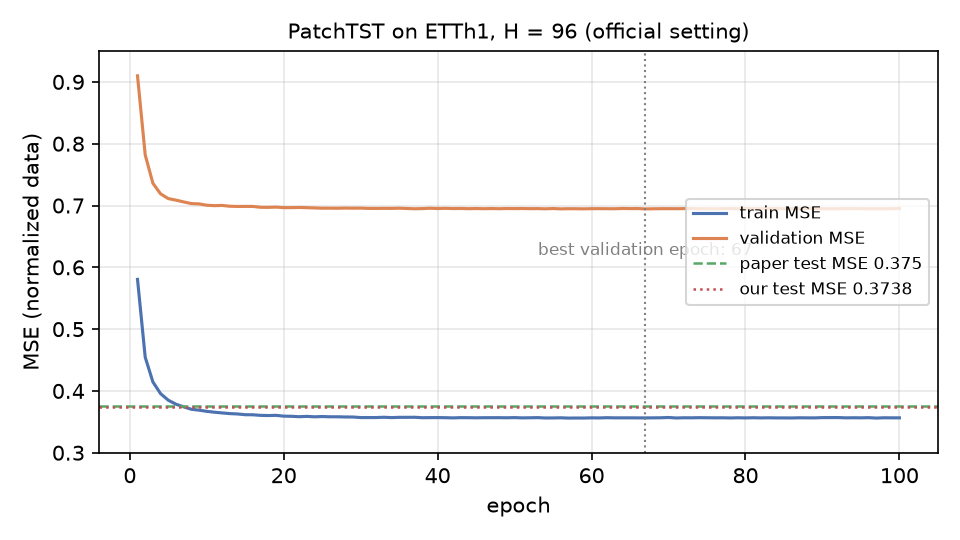
\includegraphics[width=0.55\linewidth]{etth1_h96_curve.png}
\caption{ETTh1 $H = 96$: training and validation MSE per epoch. The best validation epoch (67) is the checkpoint
that is tested; the test MSE of 0.374 is the paper's 0.375.}
\label{fig:curve}
\end{figure}

\paragraph{Ablations.} These reproduce the paper's reasoning, not just its headline number. Taking RevIN out
costs 3\% in MSE. Mixing channels costs 11\% and needs six times the parameters. Removing patching altogether, one token per time step, is 2\% more accurate, but it has $6.6\times$ the parameters and $64\times$ the
attention memory, and it would not fit on a MIG slice at all. Patching buys cost, not accuracy, which is how the
paper frames it too. The whole base-paper phase used about 22 SU.

\paragraph{Data pipeline is built and audited.} DS-01 downloads SDWPF from the Hugging Face mirror with SHA-256
checks and applies the cleaning rules. Of the 4,727,520 readings, 3,595,859 (76\%) are valid. Another 1,082,113
(23\%) are unknown, almost all of it curtailment, where the turbine reports zero power although the wind is above
cut-in speed; 49,518 are missing and 127 abnormal. 1,263,062 negative readings were clamped. DS-02 fixes the split
and, because it counts valid readings per window, revealed several problems: day
66 is a farm-wide outage with no valid readings at all, validation day 193 and test days 229 to 233 are under 25\%
valid, and the worst turbine is 67\% valid over the whole period. At $H = 6$, one in five validation windows has
no valid target. So the evaluation keeps every origin and scores per reading with a mask instead of dropping
windows. The origin lists and per-window counts are committed, which is what guarantees every model sees the
same windows. DS-03 writes each training subset and the validation period as GluonTS Arrow files, with a switch
for whether flagged readings are kept or blanked, and we confirmed on Zaratan that Chronos's unmodified
\code{train.py} loads and trains on all eight files.

\section{Challenges and changes}

\paragraph{Problems encountered.}
\begin{itemize}
  \item \textbf{Memory on MIG slices.} The no-patching ablation needs about 1.5\,GB per layer just for attention
  at 337 tokens and batch 128, and the 5\,GB slice ran out. Rather than change the recipe with gradient
  accumulation and lose comparability, we ran it once on a full A100 (19 minutes, about 15 SU).
  \item \textbf{Queue waits.} A full A100 took several hours to come through. We now keep everything that fits on
  MIG slices and submit long jobs early with checkpoint-resume.
  \item \textbf{The Chronos environment.} \code{transformers} 5.x fails to import on our \code{torch} 2.5.1, so it
  is pinned below 5. Chronos's extras pull in a newer \code{pyarrow}, so that pin became a minimum. And
  \code{train.py} only accepts options through a YAML file, which we now keep in the repository.
\end{itemize}

\paragraph{Changes from the proposal.}
\begin{itemize}
  \item \textbf{Flagged readings in inputs.} The proposal said we would gap-fill inputs by carrying the last value
  forward. We now keep unknown and abnormal readings in the inputs as real values, because the turbine did
  produce zero when it was curtailed, and we mask them only in the loss and the metrics.
  Chronos cannot make that distinction, since its training script treats a NaN as both a missing input and a
  missing target. So DS-03 exports both variants and CF-01 will run both on the 5\% subset and report the
  difference.
  \item \textbf{One model per horizon or one for all.} The paper trains a separate PatchTST per horizon. Chronos
  predicts 64 steps and we read off 6 and 36. To keep the comparison fair, PT-01 will train PatchTST the same way,
  one $H = 64$ model, and we will note the per-horizon variant as the paper's practice.
  \item \textbf{What ``validation'' means.} Early stopping and model selection use the 99 shared origins per
  turbine, not every stride-1 window. That way the validation numbers we report are the same ones that picked the
  model.
\end{itemize}

\section{Remaining work and timeline}

\begin{table}[H]
\centering\small
\caption{Plan to the final report. Dates are targets; the grid gate is the one that matters.}
\label{tab:timeline}
\footnotesize\setlength{\tabcolsep}{4pt}\begin{tabular}{@{}lp{8.2cm}ll@{}}
\toprule
Dates & Work & Owner & Items \\
\midrule
Oct 30 -- Nov 7  & Shared evaluation module; persistence and seasonal-naive baselines & Tanmay & DS-04, DS-05 \\
Oct 30 -- Nov 10 & PatchTST on SDWPF with masked loss; quantile head; head-design pilot at full data & Simran & PT-01--03 \\
Nov 8 -- Nov 14  & LSTM baseline; Chronos zero-shot on the fixed windows & Tanmay & DS-06, DS-07 \\
Nov 10 -- Nov 21 & Chronos full fine-tune (both flagged-reading variants on 5\%, then the grid); LoRA via \code{peft} & Tanmay / Simran & CF-01, CF-02 \\
Nov 17 -- Nov 24 & Slurm job array; run the 27-run grid with 3 seeds & both & EX-01, EX-02 \\
Nov 24          & \textbf{Gate:} grid finished, all results JSON committed & both & \\
Nov 21 -- Nov 28 & Optional: DDP fine-tune of Chronos-T5-base on 2 A100s, if the pool allows & Simran & CF-03 \\
Nov 25 -- Dec 2  & Analysis and plots: error vs.\ data fraction, cost vs.\ accuracy, per-horizon tables & both & EX-03 \\
Dec 3 / Dec 10   & Presentation; final report due Dec 10 & both & \\
\bottomrule
\end{tabular}
\end{table}

On compute, we expect the grid to cost about 200 SU: PatchTST runs are under 1 SU each and a Chronos-small
fine-tune is a few SU on a MIG slice. The optional T5-base runs would add up to 100 SU. We have used about 22 SU
so far.

\section{Individual contributions}

\paragraph{Simran Kharbanda.} Set up the repository, the issue and PR conventions, and the Zaratan environment
and Slurm scripts (BP-01). Implemented and verified PatchTST end to end, BP-02 through BP-06, then the three
remaining horizons and the three ablations, including the memory workaround for no-patching (BP-08). Checked the
Chronos environment on Zaratan (version pins, the \code{train.py} smoke config) for DS-01 to DS-03. Next: PT-01 to PT-03, LoRA fine-tuning (CF-02), the DDP run (CF-03), the Slurm job array
(EX-01), and the shared grid and analysis work.

\paragraph{Tanmay Sharma.} Built the data pipeline: SDWPF download, cleaning and the validity mask with
per-turbine and per-day audits (DS-01); the splits, nested subsets, fixed evaluation origins and the
window-coverage report (DS-02); and the GluonTS Arrow export with the flagged-reading switch and validation file
(DS-03). Next: the shared evaluation code (DS-04), the
baselines and the LSTM (DS-05, DS-06), Chronos zero-shot (DS-07), full fine-tuning (CF-01), the analysis (EX-03),
and the shared grid work.

\section*{References}
{\renewcommand{\section}[2]{}%
\footnotesize
\begin{thebibliography}{9}
\bibitem{nie2023patchtst}
Y.~Nie, N.~H.~Nguyen, P.~Sinthong, and J.~Kalagnanam.
\newblock A time series is worth 64 words: Long-term forecasting with transformers.
\newblock \emph{ICLR}, 2023. Code: \url{https://github.com/yuqinie98/PatchTST}

\bibitem{ansari2024chronos}
A.~F.~Ansari et~al.
\newblock Chronos: Learning the language of time series.
\newblock \emph{Transactions on Machine Learning Research}, 2024. \url{https://arxiv.org/abs/2403.07815}

\bibitem{hu2022lora}
E.~J.~Hu et~al.
\newblock LoRA: Low-rank adaptation of large language models.
\newblock \emph{ICLR}, 2022.

\bibitem{zhou2024sdwpf}
J.~Zhou et~al.
\newblock SDWPF: A dataset for spatial dynamic wind power forecasting over a large turbine array.
\newblock \emph{Scientific Data}, 11, 2024. \url{https://arxiv.org/abs/2208.04360}

\bibitem{kim2022revin}
T.~Kim et~al.
\newblock Reversible instance normalization for accurate time-series forecasting against distribution shift.
\newblock \emph{ICLR}, 2022.

\bibitem{zhou2021informer}
H.~Zhou et~al.
\newblock Informer: Beyond efficient transformer for long sequence time-series forecasting (ETTh1 dataset).
\newblock \emph{AAAI}, 2021.

\bibitem{chronosrepo}
Amazon Science.
\newblock chronos-forecasting (software, Apache-2.0).
\newblock \url{https://github.com/amazon-science/chronos-forecasting}

\bibitem{peft}
Hugging Face.
\newblock PEFT: Parameter-efficient fine-tuning (software).
\newblock \url{https://github.com/huggingface/peft}

\end{thebibliography}}

\end{document}
